\documentclass{article}
\usepackage{geometry}
 \geometry{
 a4paper,
 total={170mm,270mm},
 left=20mm,
 top=10mm,
 }
\usepackage{graphicx}
\usepackage{float}
\usepackage{enumitem}
\usepackage{caption}
\usepackage{amsmath}
\newcommand*{\addheight}[2][.5ex]{%
  \raisebox{0pt}[\dimexpr\height+(#1)\relax]{#2}%
}
\title{\textbf{Chaotic Dynamics - CSCI 5446} \\
Problem Set 10}
\author{Santhanakrishnan Ramani}
\begin{document}
\maketitle
\section*{Problem 1}
\paragraph{•}
I implemented the box-counting algorithm using \textbf{uniquetol} method (suggested by prof. in class) in matlab which is used to find the Unique values within some tolerance (which in our case is the epsilon value) given a dataset. The command that I used to find the number of boxes for a given $\epsilon$ is,\\
$$length(uniquetol(points,\epsilon,"ByRows",true,"DataScale",1))$$

\section*{Problem 2}
\begin{enumerate}[label=(\alph*)]
\item
The Figure \ref{fig:prob2a} represents the plot of $log N(\epsilon)\,\, vs\,\, log(1/\epsilon)$ for the Lorenz trajectory with $a=16, r=45, b=4$ and initial condition (-13,-12,52) for $\epsilon$ values ranging from 2 to 0.001. The shape of the plot is as expected as it initially increases and reaches a constant value when the $\epsilon$ value is less than the minimum distance between any two points. The dimension capacity was found to be 1.25.

\begin{minipage}{\linewidth}
{
\centering 
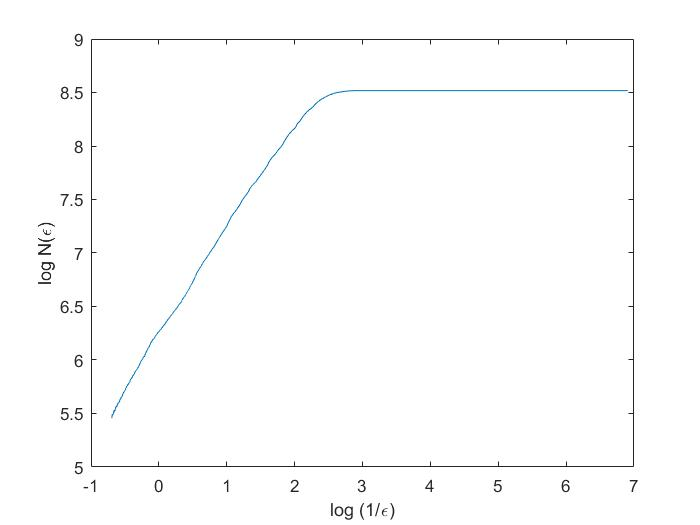
\includegraphics[scale=0.4]{images/prob2a.jpg}
\captionof{figure}{Box Counting Dimension}
\label{fig:prob2a}
}
\end{minipage}

\item
Now running the above algorithm for more steps, I see the results change, the new dimension capacity of the Lorenz trajectory was found to be 1.3. I trust the results of running for longer time steps, as it gives more clear picture of the whole system.  

\item
On performing the box counting algorithm on the set of data points that was generated using embedding dimension m=3 and $\tau=108$, I found the capacity dimension to be equal to 1.37. The plot of both the original and reconstructed trajectory looks similar, but the number of boxes needed for the same value of epsilon is higher in the reconstructed trajectory compared to the original which is expected.

\end{enumerate}
\section*{Problem 3}
\paragraph{•}
In order to avoid box/size memory limitation, we can you use efficient data structures like KD tree, linked list, Jagged arrays, Hashing techniques or by coloring the respective pixel of an image instead of using matrices, as they store just the required data and hence lesser space.

\section*{Problem 4}
\paragraph{•}
The Figure \ref{fig:prob4c} and \ref{fig:prob4d} represents the plot of $C(m,\epsilon)$ vs $\epsilon$ and $D(m,\epsilon)$ vs $\epsilon$ using TISEAN correlation dimension calculator d2 on the reconstructed trajectory for embedding dimension 3 to 7. From figure \ref{fig:prob4d} we can see a plateau at 2 for $\epsilon$ values from 0.1 to 20, which corresponds to the correlation dimension. The figure \ref{fig:prob4c} shows that the correlation sum for the different embedding dimensions remain nearly the same indicating self-similar geometry.

\begin{minipage}{\linewidth}
{
\centering 
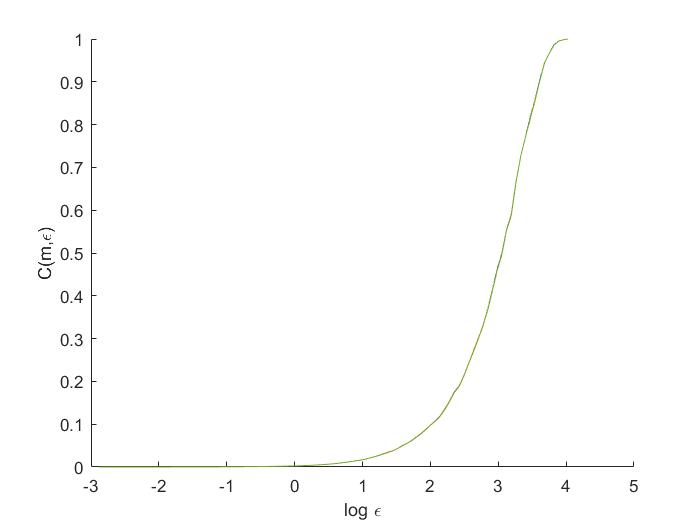
\includegraphics[scale=0.4]{images/prob4c.jpg}
\captionof{figure}{Correlation Dimension}
\label{fig:prob4c}
}
\end{minipage}

\begin{minipage}{\linewidth}
{
\centering
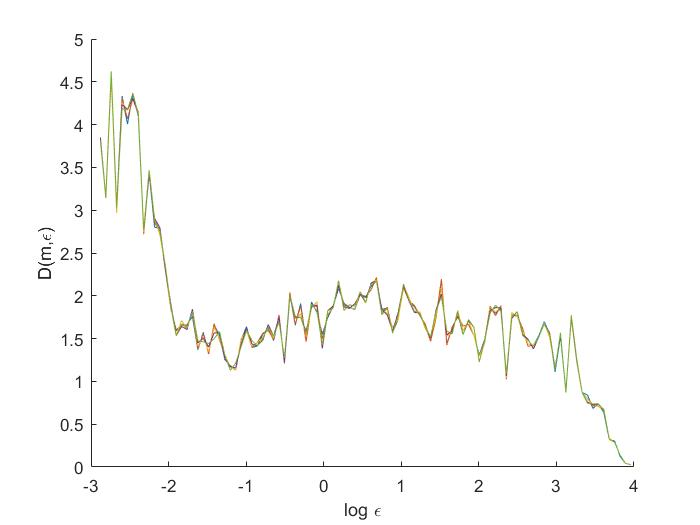
\includegraphics[scale=0.4]{images/prob4d.jpg}
\captionof{figure}{Correlation Dimension}
\label{fig:prob4d}
}
\end{minipage}
\end{document}
